%%%%%%%%%%%%%%%%%%%%%%%%%%%%%%%%%%%%%%%%%%%%%%%%%%%%%%%%%%%%%%%%%%%%
%                                                                  %
%   Copyright (c) 2010 - 2011 Caspar Zhang <casparant@gmail.com>   %
%                                                                  %
%   This copyrighted material is made available to anyone wishing  %
%   to use, modify, copy, or redistribute it subject to the terms  %
%   and conditions of the GNU General Public License version 2.    %
%                                                                  %
%   This program is distributed in the hope that it will be        %
%   useful, but WITHOUT ANY WARRANTY; without even the implied     %
%   warranty of MERCHANTABILITY or FITNESS FOR A PARTICULAR        %
%   PURPOSE. See the GNU General Public License for more details.  %
%                                                                  %
%   You should have received a copy of the GNU General Public      %
%   License along with this program; if not, write to the Free     %
%   Software Foundation, Inc., 51 Franklin Street, Fifth Floor,    %
%   Boston, MA 02110-1301, USA.                                    %
%                                                                  %
%%%%%%%%%%%%%%%%%%%%%%%%%%%%%%%%%%%%%%%%%%%%%%%%%%%%%%%%%%%%%%%%%%%%

\documentclass[a4paper,oneside,12pt]{book}
\usepackage{inc/BUPTthesisbachelor}

%%%%%%%%%%%%%%%%%%%%%%%%% Begin Documents %%%%%%%%%%%%%%%%%%%%%%%%%%
\begin{document}

%%%%%%%%%%%%%%%%%%%%%%%%%%%%%%%%%%%%%%%%%%%%%%%%%%%%%%%%%%%%%%%%%%%%
%                                                                  %
%   Copyright (c) 2010 - 2011 Caspar Zhang <casparant@gmail.com>   %
%                                                                  %
%   This copyrighted material is made available to anyone wishing  %
%   to use, modify, copy, or redistribute it subject to the terms  %
%   and conditions of the GNU General Public License version 2.    %
%                                                                  %
%   This program is distributed in the hope that it will be        %
%   useful, but WITHOUT ANY WARRANTY; without even the implied     %
%   warranty of MERCHANTABILITY or FITNESS FOR A PARTICULAR        %
%   PURPOSE. See the GNU General Public License for more details.  %
%                                                                  %
%   You should have received a copy of the GNU General Public      %
%   License along with this program; if not, write to the Free     %
%   Software Foundation, Inc., 51 Franklin Street, Fifth Floor,    %
%   Boston, MA 02110-1301, USA.                                    %
%                                                                  %
%%%%%%%%%%%%%%%%%%%%%%%%%%%%%%%%%%%%%%%%%%%%%%%%%%%%%%%%%%%%%%%%%%%%

% 你只需要修改下面几行就可以完成大部分内容的填写,
% 这要求你具有一定的LaTeX基础,但是如果你足够聪明,
% 不具有LaTeX基础也可以完成。

% 论文中文题目
\def\thesistitle{这里是毕设的题目,有时候它会被分成两行}

% 论文英文题目
\def\thesistitleen{This is the title in English Version, it will be broken into 3 lines at most if the title is long enough.}

% 封面上要填的一些项目
\def\name{张\quad{}\quad{}三} % 姓名
\def\institute{叉叉学院}      % 学院
\def\major{欧欧工程}          % 专业
\def\class{09XXX}             % 班级
\def\stuno{09XXXX}            % 学号
\def\classno{XX}              % 班内序号
\def\supervisor{老~师~好}     % 指导老师
\def\date{二〇一三~年~六~月}  % 日期 TODO:如何自动打上日期?

% Thank Words
\def\thankwords{
    感谢国家,感谢CCAV;

    感谢XXX导师对我的论文的精心指导;

    感谢你感谢我感谢他。
}
    % Main items 
%%%%%%%%%%%%%%%%%%%%%%%%%%%%%%%%%%%%%%%%%%%%%%%%%%%%%%%%%%%%%%%%%%%%
%                                                                  %
%   Modified by Bing Hsu <hello@antinucleon.com> 2013              %
%   Forked From (c) 2010 - 2011 Caspar Zhang <casparant@gmail.com> %
%                                                                  %
%   This copyrighted material is made available to anyone wishing  %
%   to use, modify, copy, or redistribute it subject to the terms  %
%   and conditions of the GNU General Public License version 2.    %
%                                                                  %
%   This program is distributed in the hope that it will be        %
%   useful, but WITHOUT ANY WARRANTY; without even the implied     %
%   warranty of MERCHANTABILITY or FITNESS FOR A PARTICULAR        %
%   PURPOSE. See the GNU General Public License for more details.  %
%                                                                  %
%   You should have received a copy of the GNU General Public      %
%   License along with this program; if not, write to the Free     %
%   Software Foundation, Inc., 51 Franklin Street, Fifth Floor,    %
%   Boston, MA 02110-1301, USA.                                    %
%                                                                  %
%%%%%%%%%%%%%%%%%%%%%%%%%%%%%%%%%%%%%%%%%%%%%%%%%%%%%%%%%%%%%%%%%%%%

\begin{titlepage}
    \centering    
    \begin{spacing}{1.05}
            % 下面的vspace支撑在Word版封面中不存在,但是由于Word版封面
            % 用了网格对齐导致排版混乱,所以加上若干vspace支撑以保持和
            % Word版封面的排版一致。无奈啊~~
            \quad{}\vspace{8mm}
            \yihao \quad{} \\
            
\includegraphics[width=12cm]{inc/buptname}\\
            \yihao \quad{} \\
            \covernamefont{本~~科~~毕~~业~~设~~计~~(论文)} \\ % thesis name
            \yihao \quad{} \\
	    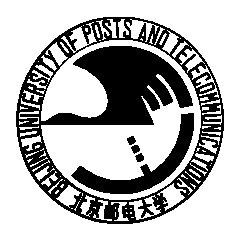
\includegraphics[width=3.5cm]{inc/buptseal}\\
            \wuhao \quad{} \\
            \parbox[c]{.7\textwidth}{%
                \thesistitlefont{题目:~~\CJKunderline*{\thesistitle}}} \\%
            \sanhao \quad{}
            \vspace{5mm}
        \end{spacing}
        \begin{spacing}{1.6}
            \coveritemsfont{姓\qquad{}名~~\ul[5cm]{\name}} \\
            \coveritemsfont{学\qquad{}院~~\ul[5cm]{\institute}} \\
            \coveritemsfont{专\qquad{}业~~\ul[5cm]{\major}} \\
            \coveritemsfont{班\qquad{}级~~\ul[5cm]{\class}} \\
            \coveritemsfont{学\qquad{}号~~\ul[5cm]{\stuno}} \\
            \coveritemsfont{班内序号~~\ul[5cm]{\classno}} \\
            \coveritemsfont{指导教师~~\ul[5cm]{\supervisor}}
        \end{spacing}
        \begin{spacing}{1.05}
            \sanhao\quad{} \\ \wuhao\quad{} \\
            \vspace{5mm}
            \coverdatefont{\date}
        \end{spacing}
\end{titlepage}
     % Cover
%%%%%%%%%%%%%%%%%%%%%%%%%%%%%%%%%%%%%%%%%%%%%%%%%%%%%%%%%%%%%%%%%%%%
%                                                                  %
%   Modified by Bing Hsu <hello@antinucleon.com> 2013              %
%   Forked From (c) 2010 - 2011 Caspar Zhang <casparant@gmail.com> %
%                                                                  %
%   Thanks for the follow persons and projects, they gave me many  %
%   helps!                                                         %
%     - cnMuggle (http://code.google.com/p/buptthesis-bachelor/    %
%     - DazzleZhang (http://code.google.com/p/buptthesis/)         %
%     - gnawux (http://code.google.com/p/latex-bupt/)              %
%     - Ruini Xue (http://sourceforge.net/projects/thuthesis/)     %
%                                                                  %
%   This copyrighted material is made available to anyone wishing  %
%   to use, modify, copy, or redistribute it subject to the terms  %
%   and conditions of the GNU General Public License version 2.    %
%                                                                  %
%   This program is distributed in the hope that it will be        %
%   useful, but WITHOUT ANY WARRANTY; without even the implied     %
%   warranty of MERCHANTABILITY or FITNESS FOR A PARTICULAR        %
%   PURPOSE. See the GNU General Public License for more details.  %
%                                                                  %
%   You should have received a copy of the GNU General Public      %
%   License along with this program; if not, write to the Free     %
%   Software Foundation, Inc., 51 Franklin Street, Fifth Floor,    %
%   Boston, MA 02110-1301, USA.                                    %
%                                                                  %
%%%%%%%%%%%%%%%%%%%%%%%%%%%%%%%%%%%%%%%%%%%%%%%%%%%%%%%%%%%%%%%%%%%%

\begin{titlepage}
    \wuhao\quad{} \\
    \begin{spacing}{1.6}
        \centering
        \statetitlefirst{北\quad{}京\quad{}邮\quad{}电\quad{}大\quad{}学} \\
        \statetitlesecond{本科毕业设计(论文)诚信声明}  \\
    \end{spacing}
    
    \normalsize
    
    \quad{}

    本人声明所呈交的毕业设计(论文),题目《\thesistitle》是本人在指导教师的指导下,独立进行研究工作所取得的成果。尽我所知,除了文中特别加以标注和致谢中所罗列的内容以外,论文中不包含其他人已经发表或撰写过的研究成果,也不包含为获得北京邮电大学或其他教育机构的学位或证书而使用过的材料。

    申请学位论文与资料若有不实之处,本人承担一切相关责任。

    \quad{} 

    本人签名:\rule[-2pt]{4cm}{1pt}\quad 日期:\rule[-2pt]{4cm}{1pt}
\end{titlepage}

 % 诚信声明
%%%%%%%%%%%%%%%%%%%%%%%%%%%%%%%%%%%%%%%%%%%%%%%%%%%%%%%%%%%%%%%%%%%%
%                                                                  %
%   Copyright (c) 2010 - 2011 Caspar Zhang <casparant@gmail.com>   %
%                                                                  %
%   This copyrighted material is made available to anyone wishing  %
%   to use, modify, copy, or redistribute it subject to the terms  %
%   and conditions of the GNU General Public License version 2.    %
%                                                                  %
%   This program is distributed in the hope that it will be        %
%   useful, but WITHOUT ANY WARRANTY; without even the implied     %
%   warranty of MERCHANTABILITY or FITNESS FOR A PARTICULAR        %
%   PURPOSE. See the GNU General Public License for more details.  %
%                                                                  %
%   You should have received a copy of the GNU General Public      %
%   License along with this program; if not, write to the Free     %
%   Software Foundation, Inc., 51 Franklin Street, Fifth Floor,    %
%   Boston, MA 02110-1301, USA.                                    %
%                                                                  %
%%%%%%%%%%%%%%%%%%%%%%%%%%%%%%%%%%%%%%%%%%%%%%%%%%%%%%%%%%%%%%%%%%%%

% 你只需要修改下面内容就可以完成中英文摘要,
% 这要求你具有一定的LaTeX基础,但是还是那句话,
% 如果你足够聪明,不具有LaTeX基础也可以完成。

% 中文摘要
\def\abstractcn{
%从这里开始写你的摘要,分段需要空一行。
这里是摘要,慢慢写,别急。最少500字。开头要空两格,在这里随便写点什么以便把这行写长超过一行。巴拉巴拉巴拉巴拉巴拉我使劲使劲巴拉。

换一段再写,测试一下分段。

这是最后一段了。
%摘要结束
}

% 中文关键字 
% TODO: 改成可变长度的
\def\abscnkeyone{关键字1}
\def\abscnkeytwo{关键字2}
\def\abscnkeythree{关键字3}
\def\abscnkeyfour{}
\def\abscnkeyfive{}

% ABSTRACT
\def\abstracten{
%Your abstract here, to make a new paragraph, give an extra blank line please.
Here is abstract, more words, more words, and more more words to break the line. Try it again. Enough?

OK, another paragraph.

The last paragraph.
%Abstract done
}

% Key Words 
% TODO: 改成可变长度的
\def\absenkeyone{Key Word 1}
\def\absenkeytwo{Key Word 2}
\def\absenkeythree{Key Word 3}
\def\absenkeyfour{}
\def\absenkeyfive{}


  % Abstract
\frontmatter\tableofcontents % Content

% 正文
\newpage\mainmatter
\fancypagestyle{plain}{\pagestyle{fancy}} % Add head to new chapter
\pagestyle{fancy} % Head and foot
%\let\cleardoublepagebak=\cleardoublepage
%\let\cleardoublepage\relax % Make new chapter stay on old page

%%%%%%%%%%%%%%%%%%%%%%%%%%%%% Main Area %%%%%%%%%%%%%%%%%%%%%%%%%%%%

\chapter{引言}
\section{使用\XeLaTeX{}+xeCJK写毕业论文}
这个模板是一个\XeLaTeX{}模板,\cite{bib:book01}使用\XeLaTeX{}
引擎编译,其中中文支持使用xeCJK\footnote{xeCJK是由孙文昌老师开
发的支持CJK文字排版的\XeLaTeX{}宏包,该宏包分高低两个版本,高
版本需要0.9995版本以上的\XeLaTeX{},texlive2008以上符合该版本
要求,而texlive2009已经自带了xeCJK宏包。}。本模板暂时只在Linux
平台上测试通过,欢迎大家在不同平台不同\TeX{}环境下编译测试。

\subsection{模板概述}
在Twitter上,@yegle同学推荐了他的同学cnMuggle(我姑且称之为梵高)
写的一个北京邮电大学本科生\LaTeX{}模板,网址在: 
http://code.google.com/p/buptthesis-bachelor/ 。但是由于梵高同
学使用的是CTeX,这是一个暂时只能在Windows上运行的工具库,作为一
个Linux用户,我只能重新发明轮子。我选择\XeLaTeX{}引擎+xecjk宏包
是因为我比较熟悉这个配置下如何使用中文。同时毕业论文对字体有要
求,而使用\XeLaTeX{}支持的Truetype字体比在\LaTeX{}下生成字体要
来得方便。

\subsection{鸣谢}
在我的模板开发过程中,主要是自己写代码,出了问题去网上搜解决方案,
\cite{bib:book02,bib:article01,bib:article02}请允许我首先不谢国
家,而谢Google和CTeX论坛,同时还要感谢前人的成果,我多多少少使用
了一些前辈的代码,他们是:

\begin{itemize}
    \item cnMuggle: http://code.google.com/p/buptthesis-bachelor/
    \item DazzleZhang: http://code.google.com/p/buptthesis/
    \item gnawux: http://code.google.com/p/latex-bupt/
    \item Ruini Xue: http://sourceforge.net/projects/thuthesis/
\end{itemize}

\chapter{模板功能性测试}
\section{滕王阁序}
首先使用我最喜欢的古文《滕王阁序\footnote{《滕王阁序》全称
《秋日登洪府滕王阁饯别序》。亦名《滕王阁诗序》,骈文名篇。唐
王勃作。}》用作测试模板。

\subsection{《滕王阁序》前三段节选}
豫章故郡,洪都新府。星分翼轸(zhěn),地接衡庐。襟三江而带五湖,
控蛮荆而引瓯越。物华天宝,龙光射牛斗之墟;人杰地灵,徐孺下陈蕃
之榻。雄州雾列,俊采星驰,台隍(huáng)枕夷夏之交,宾主尽东南之
美。都督阎公之雅望,棨(qǐ )戟(jǐ)遥临;宇文新州之懿(yì)范,
襜(chān )帷(wéi)暂驻。十旬休假,胜友如云;千里逢迎,高朋满
座。腾蛟起凤,孟学士之词宗;紫电青霜,王将军之武库。家君作
宰,路出名区;童子何知,躬逢胜饯。

时维九月,序属三秋。潦(lǎo)水尽而寒潭清,烟光凝而暮山紫。
俨(yán)骖騑(cān fēi)于上路,访风景于崇阿。临帝子之长洲,得
天人之旧馆。层峦耸翠,上出重霄;飞阁流丹,下临无地。鹤汀凫
(fú )渚,穷岛屿之萦(yíng)回;桂殿兰宫,即冈峦之体势。

披绣闼(tà),俯雕甍(méng )。山原旷其盈视,川泽纡(yū)其骇
瞩。闾阎扑地,钟鸣鼎食之家;舸舰弥津,青雀黄龙之舳(zhú)。
云销雨霁(jì),彩彻区明。落霞与孤鹜齐飞,秋水共长天一色。
渔舟唱晚,响穷彭蠡(lǐ)之滨;雁阵惊寒,声断衡阳之浦。

\subsection{滕王阁风景}
滕王阁,高耸于南昌城西,赣江之滨。实景如图\ref{fig:twg01}:
\buptfigure{inc/twg}{滕王阁实景}{fig:twg01}
步入阁中,仿佛置身于一座以滕王阁为主题的艺术殿堂。在第一层
正厅有一幅表现王勃创作《滕王阁序》的大型汉白玉浮雕《时来风
送滕王阁》,巧妙地将滕王阁的动人传说与历史事实融为一体。第
二层正厅是23.90×2.55米的大型工笔重彩壁画《人杰图》,绘有自
秦至明的80位各领风骚的江西历代名人。这与第四层表现江西山川
精华的《地灵图》,堪称双璧,令人叹为观止。第五层是凭栏骋目
的最佳处。进入厅堂,迎面是苏东坡手书的千古名篇《滕王阁
序》。每一层都有一个主题,亦都与阁有关。

\section{系统调用}

不要怪我话题转换得太快,这里要测试一下表格和其他功能,所以
就回归老本行啦。关于系统调用,有如下定义:

\begin{definition}
    In computing, a system call is how a program requests 
    a service from an operating system's kernel that it 
    does not normally have permission to run.
\end{definition}

\subsection{系统调用的分类}

通常,我们把系统调用分为8类,他们分别分类如下(见表\ref{tab:syscall01}):

\begin{bupttable}{系统调用的分类}{tab:syscall01}
    \begin{tabular}{c|c|c|c}
        \hline
        \multicolumn{2}{c|}{分类} & 数量 & 举例 \\ \hline
        \multicolumn{2}{c|}{进程控制} & 约40个 & fork \\ \hline
        \multirow{2}{*}{文件系统控制} & 文件读写操作 & TBD & open, close \\ \cline{2-4}
        & 文件系统操作 & TBD & chmod \\ \hline
        \multicolumn{2}{c|}{系统控制} & TBD & ioctl \\ \hline
        \multicolumn{2}{c|}{内存管理} & TBD & mmap \\ \hline
        \multicolumn{2}{c|}{网络管理} & TBD & gethostid \\ \hline
        \multicolumn{2}{c|}{Socket控制} & TBD & bind \\ \hline
        \multicolumn{2}{c|}{用户管理} & TBD & getuid \\ \hline
        \multirow{5}{*}{进程间通信} & 信号 & TBD & sigaction \\ \cline{2-4}
        & 消息 & TBD & msgctl \\ \cline{2-4}
        & 管道 & TBD & pipe \\ \cline{2-4}
        & 信号量 & TBD & semctl \\ \cline{2-4}
        & 共享内存 & TBD & shmctl \\ \hline
    \end{tabular}
\end{bupttable}

\section{来点数学的\cite{bib:inproceeding01}}

这里要测试的是公式。

\subsection{随机分布}

\begin{definition}
    圆对称复高斯随机向量:\cite{bib:inproceeding02}如果一个复高
    斯随机向量$\bm{X}\in C^{n}$对应的实随机向量$\bm{X}$的协方差矩
    阵具有如下形式:
    \begin{equation}
        E[(\hat{\bm{X}}-E[\hat{\boldsymbol{X}}])
        (\hat{\bm{X}}-E[\hat{\boldsymbol{X}}])^{H}]
        =\cfrac{1}{2}
        \begin{array}({cc})
            Re(\bm{Q}) & -Im(\boldsymbol{Q}) \\
            Im(\bm{Q}) & Re(\boldsymbol{Q}) \\
        \end{array}
    \end{equation}
\end{definition}


%%%%%%%%%%%%%%%%%%%%%%% Main Area ENDs Here %%%%%%%%%%%%%%%%%%%%%%%%
%\let\cleardoublepage=\cleardoublepagebak
% Reference
\clearpage\phantomsection\addcontentsline{toc}{chapter}{参考文献}
\bibliographystyle{buptbachelor}
\refbodyfont{\bibliography{ref}}

% Thanks to page
\clearpage\phantomsection\addcontentsline{toc}{chapter}{致\qquad{}谢}
\chapter*{致\qquad{}谢}
\normalsize\thankwords

% Appendix
\clearpage\phantomsection\addcontentsline{toc}{chapter}{附\qquad{}录}
\chapter*{附\qquad{}录}
%%%%%%%%%%%%%%%%%%%%%%%%%%%%%%%%%%%%%%%%%%%%%%%%%%%%%%%%%%%%%%%%%%%%
%                                                                  %
%   Modified by Bing Hsu <hello@antinucleon.com> 2013              %
%   Forked From (c) 2010 - 2011 Caspar Zhang <casparant@gmail.com> %
%                                                                  %
%   This copyrighted material is made available to anyone wishing  %
%   to use, modify, copy, or redistribute it subject to the terms  %
%   and conditions of the GNU General Public License version 2.    %
%                                                                  %
%   This program is distributed in the hope that it will be        %
%   useful, but WITHOUT ANY WARRANTY; without even the implied     %
%   warranty of MERCHANTABILITY or FITNESS FOR A PARTICULAR        %
%   PURPOSE. See the GNU General Public License for more details.  %
%                                                                  %
%   You should have received a copy of the GNU General Public      %
%   License along with this program; if not, write to the Free     %
%   Software Foundation, Inc., 51 Franklin Street, Fifth Floor,    %
%   Boston, MA 02110-1301, USA.                                    %
%                                                                  %
%%%%%%%%%%%%%%%%%%%%%%%%%%%%%%%%%%%%%%%%%%%%%%%%%%%%%%%%%%%%%%%%%%%%

%TODO: make appendix more confenient for using.

\phantomsection
%\addcontentsline{toc}{chapter}{附\quad{}\quad{}录}
%\chapter*{附\quad{}\quad{}录}
\chapter*{附\qquad{}录}

\appendix

\phantomsection
\addcontentsline{toc}{section}{附录1\quad{}这里是附录1}
\section*{附录1\quad{}这里是附录1}
关于附录1,要写一些内容。

\phantomsection
\addcontentsline{toc}{section}{附录2\quad{}这里是附录2}
\section*{附录2\quad{}这里是附录2}
关于附录2,也要写一些内容。


\end{document}
